\documentclass[12pt,a4paper]{report}

\usepackage[utf8]{inputenc}
\usepackage[T1]{fontenc}

\usepackage[toc]{glossaries}

\usepackage[backend=biber,style=verbose-trad2,,autocite=footnote,sorting=ynt,ibidtracker=constrict]{biblatex}
\usepackage{csquotes}
\usepackage{hyperref}
\usepackage{caption}
\usepackage{labels}

\usepackage[a4paper, total={7in, 10in}]{geometry}

\usepackage{graphicx, copyrightbox}
\usepackage{appendix}

\setlength{\parindent}{24pt} 


\addbibresource{bib.bib}

\usepackage[french]{babel}


\title{MR 52 : Contraception masculine}
\author{Esteban BECKER}
\date{2023}
\begin{document}
\maketitle
\tableofcontents
\chapter*{Introduction}

\begin{figure}[!htb]
    \centering
    
\includegraphics[width=0.6\textwidth]{images/intro/choisir-sa-contraception.png}
    \caption{Brochure de santé publique France sur la contraception.}
    \label{fig:brochureSPF}
\end{figure}
On peut voir sur cette brochure de santé publique France qu'il y a uniquement 2 hommes représentés face à 10 femmes. \footcite{santepublicfranceChoisirSaContraception2019}
\chapter{Les méthodes de contraception}

Il y a actuellement plusieurs méthodes de contraception disponible et en cours de développement à différents stades.

\section{Les méthodes de la Haute Autorité de Santé (HAS)}
Sur leur site, la haute autorité de santé liste 3 options de contraception masculine : le préservatif, la vasectomie et le retrait. \footcite{ContraceptionChezHomme2019}

\subsection{Le préservatif}

\begin{figure}[!htb]
    \centering
    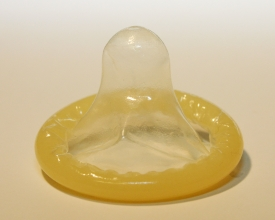
\includegraphics[width=0.3\textwidth]{images/scientiphique/Kondom.jpg}
    \caption{Préservatif masculin enroulé par User Flegmus sur pl.wikipedia — Flegmus, CC BY-SA 3.0, \href{https://commons.wikimedia.org/w/index.php?curid=1293908}{https://commons.wikimedia.org/w/index.php?curid=1293908}}
    \label{fig:preservatif}
\end{figure}

Le préservatif est une méthode de contraception consistant en un étui étanche. Il permet de séparer le sperme du vagin et ainsi d'éviter la fécondation. \footcite{PreservatifWikipedia}
De plus, il est le moyen le plus efficace de se protéger des IST (infection sexuellement transmissible). \footcite{MaladiesInfectionsSexuellement}
Le préservatif qui nous intéresse est le préservatif masculin moderne qui est principalement en latex et a été inventé en 1855. \footcite{PreservatifWikipedia}
C'est le premier moyen de contraception recommander quand on a un nouveau partenaire sexuel ou un inconnu grâce à sa protection contre les IST. \footcite{PreventionIST}
Son niveau d'efficacité théorique est de 98\% et son efficacité réelle est de 85\% selon l'indice de Pearl. L'indice de Pearl mesure l'efficacité d'une méthode de contraception, il s'agit du nombre de grossesses involontaires pour 100 femmes utilisant cette méthode pendant un an.\footcite{EfficaciteMoyensContraceptifs}
Cette différence s'explique principalement par un mauvais emplois du préservatif.
Le préservatif doit être mis avant chaque rapport. \footcite{TousMoyensContraception2023} 

\subsection{La vasectomie}

\begin{figure}[!htb]
    \centering
    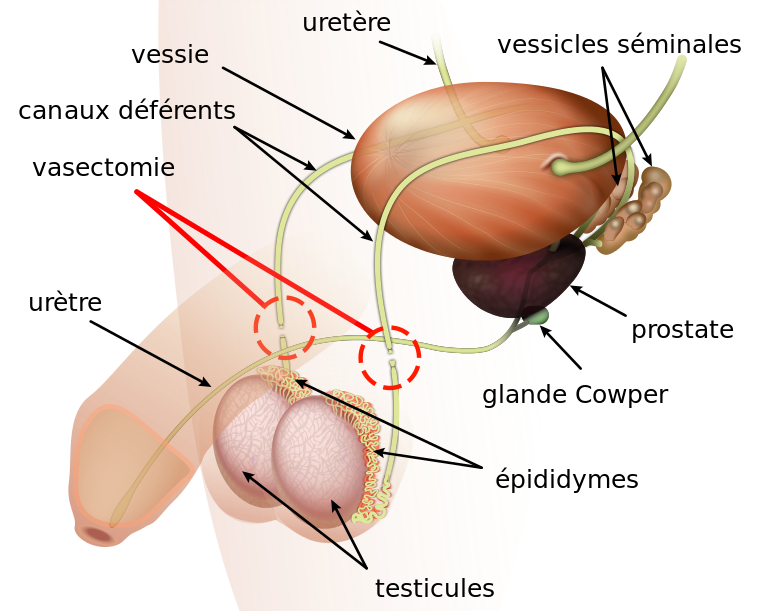
\includegraphics[width=0.5\textwidth]{images/scientiphique/Vasectomie_fr.svg.png}
    \caption{Schéma d'un pénis avec l'emplacement de la vasectomie par K. D. Schroeder, CC BY-SA 3.0, \href{https://commons.wikimedia.org/w/index.php?curid=41078528}{https://commons.wikimedia.org/w/index.php?curid=41078528}}
    \label{fig:vasectomie}
\end{figure}

La vasectomie est une méthode de contraception consistant à sectionner les canaux déférents. Il existe deux méthodes de vasectomie :
\begin{itemize}
    \item La technique classique (la méthode la plus courante) où le chirurgien effectue deux incisions au niveau du scrotum puis découpe une section des canaux déférents. Il termine l'opération par l'instalation de points de sutures ou d'agrafes \footcites{VasectomieToutSavoir2017}{guillaumedaudinContraceptesEnqueteDernier2022}
    \item La technique sans bistouri où une pince spéciale permet d'extraire les canaux par un petit trou. Ce qui permet de ne pas faire d'incisions. Ensuite les canaux sont cousus cautérisé et découpé. Cette méthode de par les plus petites ouvertures ne nécessite pas de points de sutures et diminue les risques de complication. \footcites{VasectomieToutSavoir2017}{guillaumedaudinContraceptesEnqueteDernier2022} Cela empêche les spermatozoïdes d'être présent dans le sperme mais n'a pas d'effet sur l'éjaculation.
\end{itemize}
L'opération se fait en une dizaine de minutes sous anesthésie locale. \footcite{VasectomieEstelleReversible}
La vasectomie est autorisée en France depuis 2001. \footcite{guillaumedaudinContraceptesEnqueteDernier2022} Pour effectuer une vasectomie, il faut avoir plus de 18 ans et après un délai de réflexion de 4 mois. C'est-à-dire qu'après un premier rendez-vous pour effectuer une vasectomie et où l'on a mis par écrit son souhait d'effectuer une vasectomie, il faut attendre 4 mois pour un second rendez-vous où l'on confirme son souhait d'effectuer une vasectomie. \footcite{SterilisationViseeContraceptive}
Après la vasectomie, il faut respecter un délai de 12 semaines avant d'être stérile. \footcite{associationfrancaisedurologieVasectomieContraceptive2012}. Son efficacité est de 99\% selon l'indice de Pearl. \footcite{EfficaciteMoyensContraceptifs}
Cette méthode ne protège pas des IST.

La vasovasectomie est l'opération permettant de réparer une vasectomie. Il faut savoir qu'en France le taux de réussite dans les trois premières années est de 30 à 70 \% selon l'association française d'urologie et si l'on attend plus longtemps, le taux chute. Elle est donc à considérer comme une méthode définitive.\footcite{VasectomieEstelleReversible}
Il faut savoir que la vasovasectomie est mieux réussi dans les pays où la vasectomie est plus régulièrement utilisé, en effet les médecins français ne sont pas habitué à effectuer des vasovasectomie. \footcite{guillaumedaudinContraceptesEnqueteDernier2022}


\subsection{Le retrait}

Le retrait (ou coït interrompu) est une méthode de contraception consistant à retirer le pénis du vagin avant l'éjaculation. \footcite{CoitInterrompuWikipedia}
Bien qu'efficace en théorie à 96\% elle ne l'est en pratique qu'à 78\%. \footcite{TousMoyensContraception2023}
Contrairement à une idée reçu, le liquide pré-séminale ne contient pas de spermatozoïdes s'il n'y a pas eu une éjaculation récente. \footcite{freeMaleContraceptionPrescription}
La faible efficacité vient de la difficulté à retirer le pénis au bon moment ou à une précédente éjaculation récente. \footcite{CoitInterrompuWikipedia}
Elle est donc à considérer comme une méthode peu efficace et selon les professionnels de santé avec lesquels j'ai dialogué, elle ne doit pas être utilisé comme méthode de contraception.
Cette méthode ne protège pas des IST.

\section{Les méthodes non validés par la Haute Autorité de Santé}

Pour mieux comprendre comment est validés un médicament voir l'annexe \ref{annexe:etapes_recherche}.

\subsection{La contraception hormonale masculine}

Pour comprendre comment fonctionne la contraception hormonale masculine, il faut comprendre comment fonctionne la production de spermatozoïdes.
La production de spermatozoïdes est contrôlé par l'axe hypothalamo-hypophyso-gonadique. Il s'agit de la connexion entre l’hypothalamus, l’hypophyse et les gonades. \footcite{HypothalamicPituitaryGonadal2022}
En fonction du taux de testostérone présent dans le corps l'hypothalamus va libérer des gonadotrophines (GnRH), ce qui va stimuler l'hypophyse. Qui elle a son tour va libérer l'hormone lutéinisante (LH) et l'hormone folliculostimulante (FSH).
La LH va stimuler les cellules de Sertoli pour lancer la spermatogenèse et produire des spermatozoïdes. La FSH va stimuler les cellules de Leydig pour produire de la testostérone. \footcite{abbeMaleContraception2020}

\begin{figure}[!htb]
    \centering
    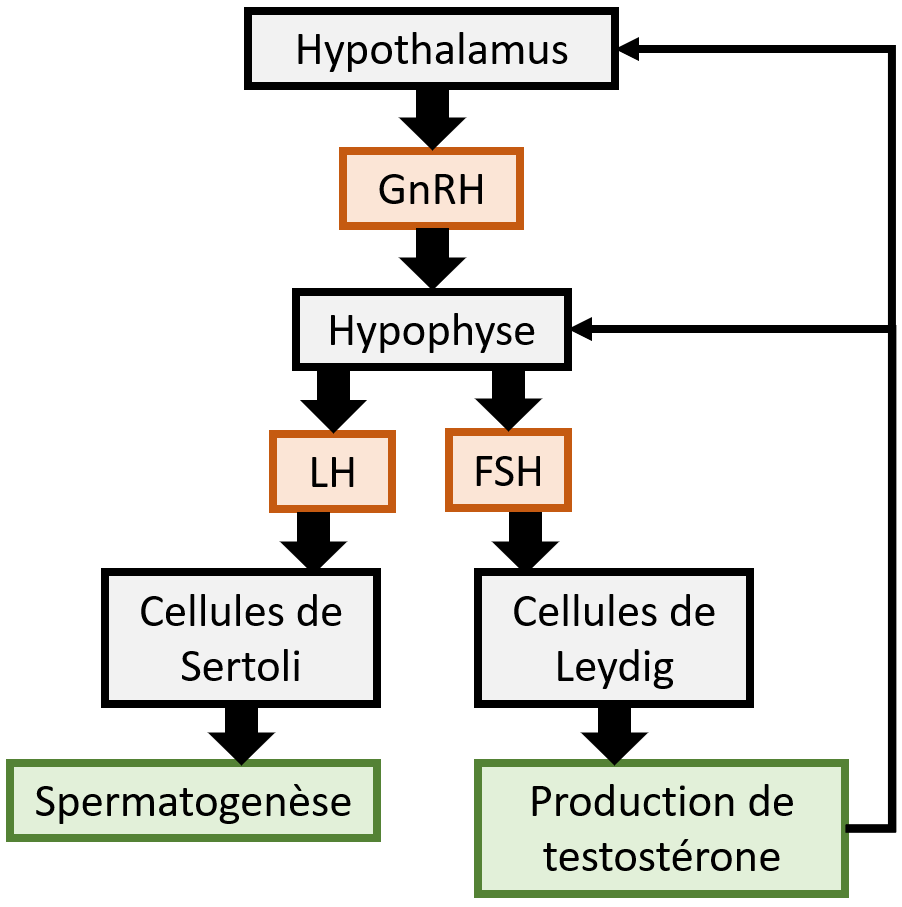
\includegraphics[width=0.4\textwidth]{images/scientiphique/axe-HPG.png}
    \caption{Schéma de l'axe hypothalamo-hypophyso-gonadique}
    \label{fig:axe-hypothalamo-hypophyso-gonadique}
\end{figure}

Ici les méthodes de contraception hormonale masculine vont viser à augmenter soit le taux de testostérone soit le taux de progestatif, ce qui va tromper l'hypothalamus et l'hypophyse et ainsi diminuer la production de spermatozoïdes. \footcite{abbeMaleContraception2020}

\begin{figure}[!htb]
    \centering
    \includegraphics[width=0.7\textwidth]{images/scientiphique/axe-HPG-contracepté.png}
    \caption{Schéma de l'axe hypothalamo-hypophyso-gonadique avec une contraception hormonale masculine}
    \label{fig:axe-hypothalamo-hypophyso-gonadique-contracepte}
\end{figure}

La spermatogenèse étant un processus long, les méthodes hormonales ont un délai minimum de 3 mois entre la première prise et la stérilité. 

\subsubsection{La contraception hormonale par injection}

Il existe plusieurs méthodes de contraception hormonale masculine par injection : \footcite{tcherdukianContraceptionMasculineQuelles2020}
\begin{itemize}
    \item L'injection intramusculaire de testostérone :
    \begin{itemize}
        \item 200 mg de testostérone hebdomadaire 
        \item 500 mg d’undécanoate de testostérone mensuelle (forme à libération prolongée) \footcite{tcherdukianContraceptionMasculineQuelles2020}
    \end{itemize}
    \item L'injection intramusculaire de testostérone et de progestatif. Le progestatif permet de diminuer la production de spermatozoïdes et la testostérone est là pour compenser la diminution de la testostérone due au progestatif. \footcite{longUpdateNovelHormonal2021}
\end{itemize}

Ainsi l'OMS a testé en 1990 l'injection intramusculaire de 200 mg d'enanthate de testostérone par semaines et dans une seconde étude de 196 avec 349 hommes. Les résultats sont positifs. En effet, sur la seconde étude l'indice de Pearson est de 1.4 grossesse. \footcite{guerinContraceptionMasculineHormonale1996}
L'OMS a donc validé cette méthode de contraception, mais elle n'a pas autorisé la mise sur le marché de ces produits. Cependant, ces produits étant déjà sur le marché pour traiter d'autres maladies. \footcite{anne-sophiedelcourHommeSousPilule} Il existe des médecins qui prescrivent ces produits pour une contraception masculine. \footcite{guillaumedaudinContraceptesEnqueteDernier2022}

\subsubsection{La contraception hormonale par voie orale}

Quand on parle de voie orale, on parle de pilule.
Cependant, contrairement aux injections, testostérone prise par voie orale est trop rapidement éliminé par le corps pour être efficace en prise quotidienne. \footcite{longUpdateNovelHormonal2021}

\subsubsection{Les effets secondaires des méthodes hormonales}

Les effets secondaires des méthodes hormonales sont :
\begin{itemize}
    \item Augmentation de la libido
    \item Augmentation de la masse musculaire ou graisseuse
    \item Agressivité
    \item Maux de tête
    \item Acné
    \item Trouble de l'humeur
    \item Dépression
    \item Calvitie précoce \footcites{guillaumedaudinContraceptesEnqueteDernier2022}{anne-sophiedelcourHommeSousPilule}{ContraceptionHormonaleMasculine2016}
\end{itemize}

Selon certains scientifiques, ces effets secondaires sont trop importants pour être utilisé comme méthode de contraception. Cependant, il est à noter que ces effets secondaires sont semblables à ceux de la contraception féminine. \footcite{ContraceptionHormonaleMasculine2016}






\listoffigures


\begin{appendix}

    \chapter{Les étapes de la recherche} \label{annexe:etapes_recherche}

    Pour mieux comprendre l'état actuel de la recherche, il faut d'abord comprendre comment est développé un médicament.
Le développement d'un médicament est divisé en plusieurs phases: \footcite{DeveloppementMedicamentInserm}

\begin{itemize}
    \item Recherche fondamentale : Il s'agit de la première étape de la recherche.
    Lors de cette étape on cherche des molécules candidates pour être utilisées comme médicament.
    On va analyser la réaction de ces molécules sur des cellules ou des tissus.
    On va sélectionner les meilleurs candidats, essayer d'améliorer leurs propriétés.

    \item Recherche préclinique : Lors de cette étape on va tester les molécules candidates sur des animaux.
    On va regarder comment elles réagissent sur des animaux, analyser s'il n'y a pas des effets secondaires, effectuer une première estimation des dosages pour l'humain.

    \item Évaluation clinique : Lors de cette étape on va tester les molécules candidates sur des humains.

    \begin{itemize}
        \item Phase 1 : On va tester la sécurité des molécules candidates sur des humains. Ici on ne teste pas l'efficacité, mais on va regarder comment elles agissent sur le corps ou si elles sont dangereuses. Les tests sont effectués sur des volontaires sains.
        \item Phase 2 : On va tester les molécules candidates sur des patients atteints de la maladie pour laquelle on cherche un médicament. De plus, plusieurs dosages seront testés pour voir lequel est le plus efficace tout en limitant les effets secondaires.
        \item Phase 3 : On va tester les molécules sur des patients malades afin d'évaluer l'efficacité du médicament. Pour cela il faut comparer l'efficacité entre les patients qui ont pris le médicament et ceux qui ont pris un placebo. Ceci permet de voir si le médicament est réellement efficace ou s'il s'agit que de l'effet placebo. En effet l'effet placebo est très puissant et peut faire croire à l'efficacité d'un médicament alors qu'il n'en a pas. \footcite{decraenPlacebosPlaceboEffects1999} Cette étape dure souvent plusieurs années.
    \end{itemize}

    \item L’autorisation de mise sur le marché (AMM) : Lors de cette étape, le laboratoire qui veut commercialiser une molécule doit demander l'autorisation de la mettre sur le marché. Pour cela il faut démontrer que le médicament est efficace et sûr. L'AMM est délivrée par l'Agence nationale de sécurité du médicament et des produits de santé (ANSM). Cette étape dure au minimum 1 an.
    \item Une fois l'AMM obtenue, le laboratoire peut commercialiser le médicament. Cependant, le médicament continue d'être surveillé au travers des retours du personnel médical, par exemple pour détecter des effets secondaires très rares.
\end{itemize}

Au total, entre le moment où une molécule est identifié par la recherche fondamentale et mis sur le marché il peut s'écouler au moins 10 ans. \footcite{DeveloppementMedicamentInserm} Du plus, a chaque étape la molécule peut être abandonnée et la recherche repart du début. \footcite{denisvanwaerebekeJamesOuRoman2018}

\end{appendix}

\printbibliography

\end{document}

